\documentclass[letterpaper,12pt]{article}

\usepackage[spanish]{babel}
\usepackage[utf8]{inputenc}
\usepackage{multirow}
\usepackage{tikz}
\usepackage{pgf-pie}
\usepackage{graphicx} % graficos
\usepackage{amsmath}
\usepackage{pgfplots}
\usepackage{textcomp}
\usepackage{siunitx}
\begin{document}
	
	\begin{titlepage}
		
		\begin{center}
			\vspace*{-1in}
			\begin{figure}[htb]
				\begin{center}
					
\includegraphics[width=8cm]{Imagen.jpeg}
				\end{center}
			\end{figure}
		
			\vspace*{0.15in}
			\begin{Large}
				\begin{center}
					\textbf{SISTEMA DE AYUDA AL DIAGNÓSTICO DE
TRASTORNOS EN ENTORNOS ESCOLARES}
				\end{center}
			\end{Large}
			\vspace*{0.3in}
			\begin{large}
				ESCUELA SUPERIOR DE INFORMÁTICA\\
			\end{large}
			\vspace*{0.3in}
			\rule{150mm}{0.1mm}\\
			\vspace*{0.6in}
			\begin{large}
				\begin{flushleft}
					{\normalsize Asignatura: Sistemas Basados en el Conocimiento}
				\end{flushleft}
				\begin{flushleft}
					{\normalsize Autores: María Blanco González-Mohíno\\} 
				\end{flushleft}
				\begin{flushleft}
					{\normalsize Fecha: Julio de 2021}
				\end{flushleft}
			\end{large}
		\end{center}
		\end{titlepage}
		\tableofcontents
		\newpage
\section{Descripción}
El objetivo principal este proyecto es desarrollar un mecanismo computacional capaz de identificar si un alumno/a sufre algún tipo de trastorno, este sistema estará enfocado para su uso por profesores ya que son estos quienes en la mayoría de casos advierten sobre una posible alteración.
El sistema contendrá una serie de reglas que desembocarán en un diagnostico hacia un alumno.

\subsection{Alcance y límites}
Este sistema distinguirá entre varios tipos de trastornos: \textit{trastornos por déficit de atención e hiperactividad, trastorno borderline, trastorno del espectro autista.}

No están incluidos cualquier otro tipo de trastorno.

\section{Estudio de viabilidad}
En este apartado se va a analizar la viabilidad del proyecto para justificar su realización. Se aplicará el test de Slager, en el que se calificarán una serie de características divididas en 4 dimensiones \textbf{(Plausibilidad, Justificación, Adecuación,
	Éxito).} Cada tarea/característica especificada puede ser esencial o deseable, a cada una de las características se le asignará un valor y un peso, el valor de las características esenciales no puede ser menor a 7, de otro modo el sistema no sería viable. Según su importancia relativa, el peso de cada característica está entre 0 y 10.
\subsection{Evaluación de la aplicación candidata}
Cada una de estas dimensiones se definirá, se le asignarán pesos a cada característica y se evaluará cada dimensión en cada respectivo subapartado.
A continuación se presenta una tabla a modo de leyenda para el entendimiento de cada tabla perteneciente a la aplicación candidata.

\begin{tabular}{|c|c|c|}
	\hline 
	Identificador & Significado & Rango \\ 
	\hline
	CAT & Categoría & ----- \\ 
	\hline 
	EX & Expertos & • \\ 
	\hline 
	TA & Tarea & • \\ 
	\hline 
	DU & Directivos o usuarios & • \\ 
	\hline 
	E & Esencial & • \\ 
	\hline 
	D & Deseable & • \\ 
	\hline 
	Pi & Característica de la dimensión de \textbf{Plausibilidad} & P1 ... P10 \\ 
	\hline 
	jI & Característica de la dimensión de Justificación & J1 ... J7 \\ 
	\hline 
	Ai & Característica de la dimensión de Adecuación & A1 ... A12 \\ 
	\hline 
	Ei & Característica de la dimensión de Éxito & E1 ... E17 \\ 
	\hline 
\end{tabular} \\

Tabla para el entendimiento de la evaluación: \\

\begin{center}
	\begin{tabular}{|c|c|}
		\hline 
		Identificador & Significado \\ 
		\hline 
		CV & Valor global de una aplicación según la dimensión \\ 
		\hline 
		Vu & Valor umbral del sistema \\ 
		\hline 
		Vp & Valor de una característica según la dimensión \\ 
		\hline 
		Pp & Peso de la característica según la dimensión \\ 
		\hline 
		Vp & Valor de una característica según la dimensión \\ 
		\hline 
	\end{tabular} \\
\end{center}
\newpage
\subsubsection{Plausabilidad}
Primera dimensión, un sistema es plausible si la tarea no requiere de sentido común y contamos con suficientes expertos con un índice de cooperatividad adecuado de modo que la tarea no nos resulte demasiado compleja. \\

Obtención de valores para el cálculo de la plausibilidad: \\
\begin{tabular}{|c|c|c|c|p{7.3 cm}|c|}
	\hline 
	CAT & IDEN. CAT & PESO & VALOR & DENOMINACIÓN DE LA CARACTERÍSITCA & TIPO \\ 
	\hline 
	EX & P1 & 10 & 8 & Existen expertos. Se tomá como expertos al profesorado del CEIP Albuera, Daimiel(Ciudad Real) & E \\ 
	\hline 
	EX & P2 & 10 & 9 & El experto asignado es genuino. & E \\ 
	\hline 
	EX & P3 & 8 & 10 & El experto es cooperativo. & D \\ 
	\hline 
	EX & P4 & 7 & 6 & El experto es capaz de articular sus métodos pero no categoriza. & D \\ 
	\hline 
	TA & P5 & 10 & 10 & Existen suficientes casos de prueba; normales, típicos, ejemplares, correosos, etc. & E \\ 
	\hline 
	TA & P6 & 10 & 9 & La tarea está bien estructurada y se entiende. & D \\ 
	\hline 
	TA & P7 & 10 & 9 & Sólo requiere habilidad cognoscitiva (no pericia física). & D \\ 
	\hline 
	TA & P8 & 9 & 8 & No se precisan resultados óptimos sino sólo Satisfactorios, sin comprometer el proyecto. & D \\ 
	\hline 
	TA & P9 & 9 & 8 & La tarea no requiere sentido común. & D \\ 
	\hline 
	TA & P10 & 7 & 9 & Los directivos están verdaderamente comprometidos con el proyecto. & D \\ 
	\hline 
\end{tabular} \\

\begin{center}
	\[
	CV_{pl} = \prod_{i=1,2,5}(Vp_{i}//Vu_{i})[\prod_{j=1}^{10}Pp_{j}*Vp_{j}]^{1/10}
	\]
	$CV_{pl} = 75,965$
\end{center}

\newpage
\subsubsection{Justificación}
Podemos saber si está justificada la realización de un sistema por diversos
motivos, unos cuantos de estos podría ser: el sistema estaría justificado si los conocimientos o experiencia del experto esté en peligro de pérdida, podría no estar justificado si no se recupera el coste de su realización. \\

Obtención de valores para el cálculo de la justificación:


\begin{tabular}{|c|c|c|c|p{7.3 cm}|c|}
	\hline 
	CAT & IDEN. CAT & PESO & VALOR & DENOMINACIÓN DE LA CARACTERÍSITCA & TIPO \\ 
	\hline 
	EX & J1 & 10 & 10 & El experto NO está disponible. & E \\ 
	\hline 
	EX & J2 & 10 & 5 & Hay escasez de experiencia humana. & D \\ 
	\hline 
	TA & J3 & 8 & 9 & Existe necesidad de experiencia simultánea en muchos lugares. & D \\ 
	\hline 
	TA & J4 & 10 & 7 & Necesidad de experiencia en entornos hostiles, penosos y/o poco gratificantes. & E \\ 
	\hline 
	TA & J5 & 8 & 7 & No existen soluciones alternativas admisibles & E \\ 
	\hline 
	DU & J6 & 7 & 4 & Se espera una alta tasa de recuperación de la inversión & D \\ 
	\hline 
	DU & J7 & 8 & 8 & Resuelve una tarea útil y necesaria. & E \\ 
	\hline 
\end{tabular} \\

\begin{center}
	\[
	CV_{ju} = \prod_{i=1,4,5,7}(Vj_{i}//Vu_{i})[\prod_{j=1}^{7}Pj_{j}*Vj_{j}]^{1/7}
	\]
	$CV_{ju} = 59,135$
\end{center}

\newpage
\subsubsection{Adecuación}
Se analiza si el problema puede resolverse con técnicas de ingeniería del conocimiento, se analiza su naturaleza, complejidad y tipo de tarea.\\

Obtención de valores para el cálculo de la adecuación: \\
\begin{tabular}{|c|c|c|c|p{7.3 cm}|c|}
	\hline 
	CAT & IDEN. CAT & PESO & VALOR & DENOMINACIÓN DE LA CARACTERÍSITCA & TIPO \\ 
	\hline 
	EX & A1 & 5 & 6 & La experiencia del experto está poco organizada & D \\ 
	\hline 
	TA & A2 & 6 & 10 & Tiene valor práctico. & D \\ 
	\hline 
	TA & A3 & 7 & 10 & Es una tarea más táctica que estratégica. No, ya que cubre necesidades actuales. & D \\ 
	\hline 
	TA & A4 & 7 & 9 & La tarea da soluciones que sirvan a necesidades a largo plazo. & E \\ 
	\hline 
	TA & A5 & 5 & 8 & La tarea no es demasiado fácil, pero es de conocimiento intensivo, tanto propio del dominio, como de manipulación de la información. & D \\ 
	\hline 
	TA & A6 & 6 & 8 & Es de tamaño manejable, y/o es posible un enfoque gradual y/o, una descomposición en subtareas independientes.Se espera poder ir añadiendo diferentes trastornos si fuese necesario. & D \\ 
	\hline 
	EX & A7 & 7 & 10 & La transferencia de experiencia entre humanos es factible (experto a aprendiz). & E \\ 
	\hline 
	TA & A8 & 6 & 7 & Estaba identificada como un problema en el área y los efectos de la introducción de un SE pueden planificarse. & D \\ 
	\hline 
	TA & A9 & 9 & 7 & No requiere respuestas en tiempo real inmediato. No es obligatorio que el resultado sea administrado en tiempo real aunque sea deseable. & E \\ 
	\hline 
	TA & A10 & 9 & 10 & La tarea no requiere investigación básica. & E \\ 
	\hline
	TA & A11 & 5 & 9 & El experto usa básicamente razonamiento simbólico que implica factores subjetivos. & D \\ 
	\hline 
	TA & A12 & 5 & 8 & Es esencialmente de tipo heurístico. & D \\ 
	\hline 
	
\end{tabular} \\

\begin{center}
	\[
	CV_{ad} = \prod_{i=4,7,9,10}(Va_{i}//Vu_{i})[\prod_{j=1}^{12}Pa_{j}*Va_{j}]^{1/12}
	\]
	$CV_{ad} = 52,012$
\end{center}

\subsubsection{Éxito}
Se determina si el sistema tendrá exito atendiendo a las cuestiones planteadas en la siguiente tabla.\\

Obtención de valores para el cálculo del éxito:

\begin{tabular}{|c|c|c|c|p{7.3 cm}|c|}
	\hline 
	CAT & IDEN. CAT & PESO & VALOR & DENOMINACIÓN DE LA CARACTERÍSITCA & TIPO \\ 
	\hline 
	EX & E1 & 8 & 10 & No se sienten amenazados por el proyecto, son capaces de sentirse intelectualmente unidos al proyecto. & D \\ 
	\hline 
	EX & E2 & 6 & 10 & Tienen un brillante historial en la realización de esta tarea. & D \\ 
	\hline 
	EX & E3 & 5 & 8 & Hay acuerdos en lo que constituye una buena solución a la tarea. & D \\ 
	\hline 
	EX & E4 & 5 & 8 & La única justificación para dar un paso en la solución es la calidad de la solución final. & D \\ 
	\hline 
	EX & E5 & 6 & 5 & No hay un plazo de finalización estricto,ni ningún otro proyecto depende de esta tarea. & D \\ 
	\hline 
	TA & E6 & 7 & 10 & No está influenciada por vaivenes políticos. & E \\ 
	\hline 
	TA & E7 & 8 & 5 & Existen ya SS.EE. que resuelvan esa o parecidas tareas. & D \\ 
	\hline 
	TA & E8 & 8 & 7 & Hay cambios mínimos en los procedimientos habituales. & D \\ 
	\hline 
	TA & E9 & 5 & 10 & Las soluciones son explicables o interactivas. & D \\ 
	\hline 
\end{tabular} \\

\begin{tabular}{|c|c|c|c|p{7.3 cm}|c|}
	\hline 
	CAT & IDEN. CAT & PESO & VALOR & DENOMINACIÓN DE LA CARACTERÍSITCA & TIPO \\ 
	\hline 
	EX & E10 & 7 & 9 & La tarea es de I+D de carácter práctico, pero no ambas cosas simultáneamente. & E \\ 
	\hline 
	EX & E11 & 6 & 10 & Están mentalizados y tienen expectativas realistas tanto en el alcance como en las limitaciones. & D \\ 
	\hline 
	EX & E12 & 7 & 10 & No rechazan de plano esta tecnología. & E \\ 
	\hline 
	EX & E13 & 6 & 9 & El sistema interactúa inteligente y amistosamente con el usuario. & D \\ 
	\hline 
	EX & E14 & 9 & 8 & El sistema es capaz de explicar al usuario su razonamiento. & D \\ 
	\hline 
	TA & E15 & 8 & 10 & La inserción del sistema se efectúa sin traumas; es decir, apenas se interfiere en la rutina cotidiana de la empresa. & D \\ 
	\hline 
	TA & E16 & 6 & 9 & Están comprometidos durante toda la duración del proyecto, incluso después de su implantación. & D \\ 
	\hline 
	TA & 17 & 8 & 9 & Se efectúa una adecuada transferencia tecnológica. & E \\ 
	\hline 
\end{tabular} \\
\begin{center}
	\[
	CV_{ex} = \prod_{i=6,10,12,17}(Ve_{i}//Vu_{i})[\prod_{j=1}^{17}Pe_{j}*Ve_{j}]^{1/17}
	\]
	$CV_{ex} = 56,325$
\end{center}
\newpage
\subsection{Evaluación global las dimensiones de la aplicación}
Para la evaluación final extraemos la media de todas las aplicaciones candidatas: 
\begin{center}
	\[
	CV = \sum_{i=1}^{4}VC_{i}/4
	\]
	$CV = 60,85925$
	\\
	Porcentaje de viabilidad, normalización del resultado:
	\begin{equation}
	\textit{Viabilidad} = \dfrac{CV*100}{CVmax} 
	\end{equation}\\
	
	CVmax = 76,21125 
	\begin{equation}
	\textit{Viabilidad} = \dfrac{61,28775*100}{76,21125} = 79,855 %
	\end{equation}
	
\end{center}

El proyecto es viable.\\
\newpage
\section{Adquisición de conocimiento}
	En este archivo solo se muestra la información obtenido a partir de la entrevista 1 hacia un docente del C.E.I.P Albuera (Daimiel), iteración número 1.
	
	\subsection{Recopilación de la primera iteración}
	\begin{flushleft}
	\textbf{Fecha: }13/03/2021 \\
	\textbf{Hora: }12:00 - 13:30 \\
	
	\end{flushleft} 
	\begin{flushleft}
	\textbf{Asistentes: } \\
	\end{flushleft}
	Experta: María de las Cruces González-Mohíno Garzás\\
	Ingeniera: María Blanco González-Mohíno
	
	\begin{flushleft}
	\textbf{Lugar:} Sala de reuniones en el C.E.I.P Albuera (Daimiel)
	\end{flushleft}
	\begin{flushleft}
	\textbf{Modo:} Entrevista no estructurada sin conocimiento previo.
	\end{flushleft}
	\begin{flushleft}
	\textbf{Objetivos de la sesión:}
	\end{flushleft}
	Esta entrevista se enfoca a dos objetivos claramente distinguidos: \\
	
	\begin{flushleft}
	1) Conocer el modo de trabajo seguido en el centro e informar adecuada-
mente de cuales serán los procedimientos a seguir para la correcta realización
del sistema. \\
	2) Extraer el conocimiento necesario para los \textit{trastornos de deficiencia
cognitiva y el trastorno del espectro autista}.
	\end{flushleft}
	
	\textbf{Fuente de conocimiento: }Profesora de infantil	
	Esta elección se ha realizado debida a la amplia experiencia en el centro Albuera (12 años) cumplimentando asi el objetivo número 1, y por la amplia
experiencia en el trabajo con niños con trastornos, objetivo número 2. \\

\textbf{Planteamiento de la sesión resultado de la sesión}
Batería de preguntas y respuestas desde una visión más general a una más
específica: \\
Repaso del proyectó a realizar para la correcta comprensión del mismo,
después, dio comienzo la entrevista: \\
	
	\textbf{*Las respuestas de las preguntas se encuentran resumidas para
evitar la extensión innecesaria del documento. Se encuentran
incluidas las partes más relevantes que aportan datos
significativos.} \\

\textit{1.- Primero me gustaría hablar un poco sobre su trabajo, sobre el modo de evaluación empleado a niños entre 3 y 5 años para la deteccion de algún
trastorno en su centro, ¿usa algún tipo de escala de evaluación, o
simplemente emplea observación sistemática?}\\

En infantil todos los profesores del centro utilizan escalas de observación
aprobadas por el inspector. Primero evalúan el sistema sensorial (3 años),
fundamentalmente la vista y el oído para encontrar niños con problemas
morfológicos, como el mal enfoque visual, niños daltónicos, etc. El oído es
fundamental para detectar un trastorno de deficit de atención mediante el
tiempo que ellos prestan atención.\\

\textit{2.- En cuanto a esto último, ¿cuánto tiempo cree que es el necesario para porder decir que el niño sufre un trastorno de deficit de atención?}\\

A edades tempranas es más difícil de determinar, un niño con déficit de
atención no permanece sentado.\\

\textit{3.- Para entrar un poco más en materia y relativo a estas edades, tengo entendido que has trabajado con niños con autismo e incluso derivado por
creer que un niño lo tenía y al contrario, hablamos de un caso en el que un
psiquiatra certificó un trastorno autista de libro en un niño y pensaste que
ese niño no era autista, ¿podría exponer el caso?}\\

El niño no centraba la mirada, típico rasgo de niño autista, pero leía a edades muy tempranas aunque solamente emitía las vocales con la entonación de la palabra, el niño también asociaba los elementos leídos a objetos materiales
y entendía la mayoría de cosas que se le decían, a parte de esto el niño era
empático con sus compañeros. No tenía la atracción por el vacío típica de
personas con este trastorno.\\

\textit{4.- Tengo entendido que la etapa gráfica de los niños también es muy
importante a la hora de detectar algo tipo de trastorno, ¿por qué?} \\

Es cierto, también se puede identificar un niño sobredotado. Los niños
borderline suelen quedarse atrasados en algunas etapas gráficas. \\

\textit{5.- Esto esta ligado a las etapas de comprensión y expresión del niño?} \\
Se puede dar en algunos casos, los niños con algún retraso podrían que-
darse atrás en estas etapas. Se les da información corta y concisa. Si el niño
no es capaz de retener información podría ser comportamiento de alguna
deficiencia cognitiva o déficit de atención. \\

\textit{6.- Si un niño no presenta un juego simbólico, a edades en las que sus
compañeros lo han alcanzado, ¿podría presentar ese niño algún trastorno?} \\

Si, en la psicología evolutiva en la fase de 3 a 6 años se tiene que dar un
juego simbólico, se emplea la técnica del juego en paralelo en niños de 3 años, de esta edad hasta los 6 si no pasan a la fase de juego simbólico podríamos estar hablando de un niño con trastorno autista ya que estos no presentan este tipo de juego. \\

\textit{7.- Vamos a cambiar un poco la linea a la deficiencia cognitiva y el retraso madurativo, ¿utilizais alguna técnica para marcar la linea entre una y otra?} \\

Se le tiene que dar un margen de evolución al niño para que sea capaz
de llegar a los diferentes niveles que ha de alcanzar en la etapa de infantil, si el niño no alcanza los niveles cuando sus compañeros están muy avanzados
podríamos estar hablando de un deficiencia cognitiva, en este caso se emplean
una serie de test, por el contrario, si el niño avanza favorablemente, aunque
vaya más lento que sus compañeros podríamos estar hablando de un retraso
psicoevolutivo.
Aún así se hace un test en la edad de los 5 años. \\

\textit{8.- ¿Cómo detectaría a un borderline estando segura que no tiene un retraso psicoevolutivo?} \\

Mediante test de inteligencia. Hay diferentes factores que influyen, en
general un borderline no es capaz de jugar con sus compañeros, ya que no
entiende las reglas del juego. Por su edad cronológica en relación a la etapa
en la que se encuentra no son capaces de adquirir los contenidos relacionados
a esa edad, si hay esta serie de comportamientos se le pasa el test, aunque
también pueden ser problemas de memoria o de inteligencia. En las etapas
gráficas no suelen llegar a la etapa del renacuajo y no hay conservación de la
materia en el niño. \\

\textit{9.- ¿Cuáles son los factores que te hacen tomar la determinación de
informar a la psicóloga del centro de que un niño tiene una deficiencia
cognitiva más grave?} \\

Hay numerosos factores, el niño no es capaz de imitar, tiene un lenguaje
muy básico, cuando un niño al finalizar infantil tiene un promedio de 2000
palabras en su vocabulario, no empatiza, no controla sus emociones, su desplazamiento no es normal.
Se ve alterado todo, desde su motricidad gruesa. Algunos no son capaces
de comer solos, retener varias ordenes.
En cambio los borderlines no suelen resolver problemas sencillos, pero su
motricidad gruesa no se ve muy afectada, también suelen presentar ecolalia. \\

\textit{10.- Ha hablado de una serie de niveles que los niños han de alcanzar,
quién marca y como están marcados estos niveles y lo que se ha de
conseguir en cada uno de ellos?} \\

El sistema educativo español está basado en las etapas de Vygotsky y
Piaget. Hay tres posibles factores: el niño lo consigue, no lo consigue y está
en proceso. \\

\textit{11.- Hemos hablado del trastorno autista, deficiencias cognitivas y
borderlines, ¿podría englobarlo en trastornos más globáles?} \\

\begin{flushleft}
Deficiencia cognitiva - Trastorno mental.\\
Trastorno del espectro autista - Trastorno neurobiológico.\\
Borderline - Afección mental.\\
\end{flushleft}

\textbf{Plan de análisis} \\
\begin{itemize}
    \item Asociación de comportamientos con sus respectivos trastornos
    \item Identificación de términos de la entrevista
    \item Generación de glosario
\end{itemize}
Se van a tratar de delimitar los términos provenientes de:\\
- Trastornos neurobiológicos.\\
- Trastornos mentales.\\
- Afecciones mentales.\\
Trataremos de delimitar los comportamientos asociados a esta
recopilación de trastornos a gran escala para poder delimitar los
comportamientos de cara a siguientes entrevistas. \\
\textbf{Resultados del análisis} \\
\textit{\textbf{• Identificación de las acciones del profesorado}}
\begin{flushleft}
Documentación de comportamientos del niño en escalas de observación. \\
Observación sistemática del niño. \\
Derivación por parte del profesorado a la psicóloga con un diagnóstico. \\
\end{flushleft}
\textit{\textbf{• Asociación de comportamientos con sus respectivos trastornos}}

Trastorno neurobiológicos: \\
- Focalización. \\
- Atracción por el vacío. \\
- Juego simbólico. \\
- Percepción de emociones. \\
- Empatía. \\
--------------------------------------------------------------------- \\
Trastorno mental: \\
- Comprensión. \\
- Juego simbólico. \\
- Adquisición de conocimiento. \\
- Etapa del renacuajo. \\
- Retención de información. \\
- Imitación. \\
- Palabras promedio. \\
- Motricidad gruesa alterada. \\
--------------------------------------------------------------------- \\
Afección mental: \\
- Resolución de problemas sencillos.\\
- Motricidad gruesa.\\
- Ecolalia.\\
- Percepción de emociones.\\

\begin{flushleft}
\textbf{Comentarios} \\
Se han encontrado muy similares los comportamientos realizados por niños
con diferentes trastornos, en la siguiente entrevista se han de concretar los
diferentes comportamientos que marcan la diferencia entre trastornos.\\
\end{flushleft}


\subsection{Recopilación de la segunda iteración}
\begin{flushleft}
En esta iteración se realizó un cuestionario a 20 profesores del CEIP Albuera y CEIP Calatrava, Daimiel, Ciudad Real. La encuesta fue totalmente anónima y vía online debido al COVID-19. 

\end{flushleft}
\begin{flushleft}
Esta encuesta estaba enfocada a concretar algunos datos de la entrevista anterior y a extraer conocimientos del trastorno TDAH. 
\end{flushleft}
\begin{flushleft}

Se realizaron diferentes secciones de preguntas:
\end{flushleft}
\begin{itemize}
\item Sobre entrevista a experto anterior
\item Sobre TDAH
\item Experiencias personales
\end{itemize} 
\newpage
\begin{flushleft}
\textbf{Cuestionario y respuestas:} \\
\textbf{Sobre entrevista anterior:} \\
\textit{1.- ¿Qué entiende con el término 'borderline'?}\\
\end{flushleft}
\begin{center}
\begin{tikzpicture}
\pie{10.5/Respuesta 2,
    78.9/Respuesta 1,
    5.3/Respuesta 3,
    5.3/Respuesta 4}
\end{tikzpicture} \\
\end{center}
\begin{itemize}
\item \emph{Respuesta 1}: Término utilizado por los expertos parade finir a un niño próximo a la deficiencia. \\
\item \emph{Respuesta 2}: El trastorno borderline se caracterizapor la inestabilidad en los estados deánimo, comportamiento y relacionesinterpersonales de quien lo padece.\\
\item \emph{Respuesta 3}: No lo conocia. \\
\item \emph{Respuesta 4}: Alumnos con una discapacidad intelectual límite. \\
\end{itemize}

\newpage
\begin{flushleft}
\textit{2.- ¿Diría que un niño que presenta discapacidad cognitiva desarrolla empatía?}\\
\end{flushleft}
\begin{center}
 \begin{tikzpicture}
\pie{94.7/Si,
    5.3/No}

\end{tikzpicture}
\end{center}

\begin{flushleft}
\textit{3.- Señala los comportamientos que opina que un niño con deficiencia cognitiva presenta}\\
\end{flushleft}
Todas las respuestas señaladas:

\begin{itemize}
\item No comprende órdenes a los 4 años
\item No presenta juego simbólico al terminar infantil
\item No adquiere conocimientos asociados a su edad cronológica
\item Estancado en la etapa del renacuajo (Etapa encontrada dentro de la etapa gráfica preesquemática)
\item No retiene información
\item No imita
\item Vocabulario reducido
\item Motricidad gruesa alterada
\item Un profesor escribió: ``Todo lo anterior''
\end{itemize}

\begin{flushleft}
\textbf{Sobre TDAH:}
\end{flushleft}
\textit{4.- ``Un niño con déficit de atención (TDAH), por lo general, presenta una conducta hiperactiva o impulsiva'' Responda si cree verdadera o falsa esta afirmación}\\

\begin{center}
 \begin{tikzpicture}
\pie{63.2/Verdadera,
    36.8/Falsa}

\end{tikzpicture}
\end{center}
\textit{5.- En su centro, si un niño presenta TDAH, ¿son capaces de dividir el tipo de déficit de atención que el niño presenta?}\\

\begin{center}
 \begin{tikzpicture}
\pie{72.2/Si,
    27.8/No}

\end{tikzpicture}
\end{center}
\textit{6.- Si su respuesta anterior fue VERDADERA conteste la siguiente pregunta: Indique en que subtipos de TDAH se divide este trastorno en su centro}\\

\begin{tikzpicture}
\begin{axis}[
xbar, xmin=0,
width=12cm, height=6cm, enlarge y limits=0.2,
xlabel={Profesores que han respondido},
symbolic y coords={Falta de atención predominante, Conducta hiperactiva/impulsiva, Combinado},
nodes near coords, nodes near coords align={horizontal},
]
\addplot coordinates {(6,Falta de atención predominante) 
(4,Conducta hiperactiva/impulsiva)
(11,Combinado)};
\end{axis}
\end{tikzpicture}
\newpage
\begin{flushleft}
\textbf{Sobre experiencias personales:}\\
\end{flushleft}
\textit{7.- Cuando ha tenido a un niño con algún tipo de trastorno, ¿Cómo lo ha identificado? Nombra el tipo de trastorno y los diferentes comportamientos seguidos por el niño, puede tener tantos ejemplos como quiera.}

\begin{flushleft}
Respuestas que respondían a la pregunta:\\
\end{flushleft}

\begin{flushleft}
\emph{Primer profesor a responder: }\\
``Dentro del espectro autista es la falta de interacción  con su entorno .
Su mirada perdida, aleteo, balanceos corporales y la necesidad de seguir unas rutinas diarias que si se alteran producen en estos niños una reacción desproporcionada y negativa. Si alteras el orden de sus rutinas pueden tener rabietas algunas veces muy intensas.
En los niños con retraso cognitivo es su falta de simbolismo que repercute tanto en su lenguaje ,comprensivo y expresivo, como en su capacidad para resolver problemas de su entorno cotidiano( subirse a una silla para alcanzar algo) , en su lógica-matemática, en sus producciones plásticas, en su motricidad gruesa y fina.
Poseen una memoria muy limitada tanto en el corto como en el medio y largo plazo
No presenta interés ni curiosidad por nada , resulta muy difícil motivarles'' \\
\end{flushleft}

\begin{flushleft}
\emph{Segundo profesor a responder: }\\
``Déficit de atención , llamadas constantes de atención , dificultad para relacionarse, escasas habilidades sociales , escasa interacción con los demás, hábitos muy mecánicos , aleteo de manos , balanceo sobre sí mismos''
\end{flushleft}

\begin{flushleft}
\emph{Tercer profesor a responder: }\\
``Tea, falta de interacción conjunta, comportamientos restringidos, no flexibilidad cognitiva''
\end{flushleft}

\begin{flushleft}
\emph{Cuarto profesor a responder: }\\
``Lo he identificado al comprobar una actividad distinta al resto de niños de su edad. TDAH: falta de atención, impulsividad no controlada, trabajos sin terminar y con graves errores, etc.''
\end{flushleft}

\begin{flushleft}
\emph{Quinto profesor a responder: }\\
``TDH, incapacidad para concentrarse, impulsividad o distracción''
\end{flushleft}

\begin{flushleft}
\emph{Sexto profesor a responder: }\\
``Trastorno cognitivo grave \\
Los comportamientos: lenguaje casi inexistente, incapacidad casi total de razonamiento, incapacidad casi total para aprender. Nula capacidad de relación social, dificultades motrices importantes. Afectación importante del plano motor,lingüístico, social, afectivo y cognitivo''
\end{flushleft}
\textit{8.- ¿Qué trastorno opina que es el más difícil de identificar desde el punto de vista docente?}\\

\begin{flushleft}
Respuestas recogidas:
\end{flushleft}

\begin{itemize}
\item Trastorno cognitivo: 1 profesor
\item Dislexia: 1 profesor
\item TLP: 1 profesor
\item Asperger: 2 profesores
\item TDAH: 4 profesores
\item TEA: 3 profesores\\
\end{itemize}

\begin{flushleft}
\textbf{Análisis de la entrevista}
\end{flushleft}
\begin{flushleft}
Modificaciones y afirmaciones que se deben llevar a cabo sobre la última iteración:
\end{flushleft}
\begin{itemize}
\item Uso del término borderline de manera correcta en relación a las demás iteraciones.
\item Borramos 'empatía' como comportamiento presentado por niños con discapacidad cognitiva.
\item Comportamientos de niños con deficiencia cognitiva correctos.
\end{itemize}

\begin{flushleft}
Comportamientos de niños con TDAH:
\end{flushleft}
\begin{itemize}
\item Conducta impulsiva o hiperactiva.
\end{itemize}

\begin{flushleft}
Es necesario concretar los diferentes niveles de TDAH en siguientes iteraciones.
\end{flushleft}

\begin{flushleft}
Comportamientos a incluir según diferentes experiencias de distintos profesores:
\end{flushleft}

\begin{flushleft}
\textit{TEA:}\\
\end{flushleft}
\begin{itemize}
\item Balbuceo.
\item Falta de interacción con su entorno.
\item Mirada perdida.
\item Aleteos.
\item Balanceos corporales.
\item Necesidad de rutinas diarias con malas reacciones derivadas de la alteración.
\item Sin flexibilidad cognitiva.
\end{itemize}
\begin{flushleft}

\textit{TDAH:}\\
\end{flushleft}
\begin{itemize}
\item Falta de atención.
\item Trabajos sin terminar.
\item Impulsividad no controlada.
\item Errores graves.
\item Incapacidad de concentrarse.

\end{itemize}

\subsection{Recopilación de la tercena iteración}
\begin{flushleft}
	\textbf{Fecha: }23/04/2021 \\
	\textbf{Hora: }17:30 - 19:45 \\
	
	\end{flushleft} 
	\begin{flushleft}
	\textbf{Asistentes: } \\
	\end{flushleft}
	Expertas: María de las Cruces González-Mohíno Garzás\\
			  Psicóloga del centro C.E.I.P Albuera
	Ingeniera: María Blanco González-Mohíno
	
	\begin{flushleft}
	\textbf{Lugar:} Sala de reuniones en el C.E.I.P Albuera (Daimiel)
	\end{flushleft}
	\begin{flushleft}
	\textbf{Modo:} Entrevista estructurada con conocimiento previo.
	\end{flushleft}
	\begin{flushleft}
	\textbf{Objetivos de la sesión:}
	\end{flushleft}
	Profundizar en el trastorno del espectro autista y asegurar los conocimientos obtenidos en anteriores iteraciones: \\
	
	\begin{flushleft}
	1) Profundizar en el trastorno del espectro autista, especialidad de la psicóloga. \\
	2) Asegurar algunos de los comportamientos en diferentes trastornos obtenidos de entrevistas anteriores.
	\end{flushleft}
	
	\textbf{Fuente de conocimiento: }\\
	\begin{itemize}
	\item Profesora de infantil:	Esta elección se ha realizado debido a la amplia experiencia en el campo de la enseñanza. Esta experta también trabajó en un centro de niños con diferentes capacidades intelectuales y trastornos.
	\item Psicóloga del centro: especializada en el trastorno del espectro autista, el cual se llevará a cabo en esta iteración.
	\end{itemize}
	

\textbf{Planteamiento y resultado de la sesión}
Batería de preguntas y respuestas. \\
	
	\textbf{*Las respuestas de las preguntas se encuentran resumidas para
evitar la extensión innecesaria del documento ya que la entrevista puede resultar demasiado larga. Se encuentran incluidas las partes más relevantes que aportan datos
significativos.} \\

\begin{flushleft}
\textbf{SOBRE TEA}
\end{flushleft}
\textit{1.- La manifestación del TEA varía según el momento de vida en el que se encuentra cada persona, pero, ¿podrían concretarse una serie de características comunes del TEA en cada etapa?}\\

No hay dos personas que presenten los mismos comportamientos ante este trastorno. \\
Comportamientos generalizados: meticulosidad, honestidad, sinceridad, atención por detalles, muy lógicos, no presentan prejuicios, buenos en tareas mecánicas y repetitivas, buen seguimiento de rutinas, conocimiento especializado sobre temas de su interes pero estos temas son muy específicos.\\

Para niños a partir de 3 años:
\begin{itemize}
\item Alteración de la comunicación: déficit en el desarrollo del lenguaje, especialmente en la comprensión, escaso uso del lenguaje, pobre respuesta a su nombre, mala comunicación no verbal (no señalar, no aguantar la mirada).

\item Alteraciones sociales: imitación limitada (no aplauden, por ejemplo), ausencia de juegos con juguetes o con otros objetos, no enseña objetos a los demás, no socializan/acercan a niños/as de su edad, no realiza juegos de ficción, no presenta juego simbólico.

\item Alteración de los intereses, actividades y conductas: mal acoplamiento a cambios, pueden presentar hipersensibilidad a los sonidos y al tacto de otras personas, muerden, pegan, agreden a iguales, oposición al adulto. Algo muy significativo: aleteos.
\end{itemize}

\textit{2.- Tengo entendido que las personas con un alto grado de autismo pueden llegar a comunicarse, intuyo que esta comunicación es muy simple, ¿se conoce algún caso de alguien con una perfecta comunicación con un alto grado de autismo?}\\

De momento no, lo normal es que no ocurra, sería raro que ocurriese, normalmente un niño de entre 3-5/6 años con TEA no se comunica si no es para pedir o rechazar, no suele comunicarse para realizar comentarios.  \\

\textit{3.- ¿Cuáles diría que son los principales factores psicomotrices de un niño con TEA, aparte del aleteo?}\\

No mira a la cara o a los ojos sonriendo a la vez.
En general sus movimientos son muy extraños y repetitivos; tiene rabietas y se resiste ante cambios ambientales; también se ríen y lloran sin motivos aparentes.\\

\textit{4.- ¿Presentaría algún tipo de juego el niño a la edad de los 3 años en adelante aunque este fuese no simbólico?}\\

No, el niño de 3 a 5/6 años presentaría juegos repetitivos, ``rituales de ordenación'' en el que ordena o alinea cosas innecesariamente. \\

\textit{5.- ¿Estos niños, presentarían ecolalia?}\\

Sí, no comprenden ni expresan conceptos abstractos, no pueden conversar, hacen preguntas escasas y repetitivas, algunos combinan 2 o 3 palabras y otros repiten estructuras que han escuchado muchas veces ya sean de la radio, TV, sus padres...

\begin{flushleft}
\textbf{SOBRE CONOCIMIENTOS ANTERIORES}
\end{flushleft}
\textit{6.- Sería correcta los siguientes niveles de TDAH: combinado, conducta hiperactiva o impulsiva y falta de atención predominante} \\

Si.\\

\textit{7.- ¿Cuál sería la forma más acertada de llamar al TEA, Trastorno del espectro autista o Trastorno Generalizado del Desarrollo?} \\

TEA, Trastorno del Espectro Autista, antes se encontraba incluido en el Trastorno Generalizado del Desarrollo, hoy día es un trastorno aparte.

\subsection{Recopilación de la cuarta iteración}

\textbf{Fecha}: 29/04/2021 \\
\textbf{Hora}: 17:30-20:00 \\
\textbf{Asistentes}: \\
Psicóloga del centro vía Teams.\\
Maria Blanco González-Mohíno. \\

\textbf{Fuentes de conocimiento} \\
Conocimientos adquiridos de las anteriores entrevistas e información recibida de la psicóloga por medio de tests y libros sobre el autismo y el trastorno de hiperactividad. \\

\textbf{Objetivos} \\
	Refinar los conocimientos adquiridos ya que podrían ser muy generales, intentar sintetizar los trastornos para la agrupación de comportamientos. \\
	
\textbf{Modo} \\
Entrevista parcialmente estructurada, intentó seguirse un orden secuencial aunque a veces se volvió a temas anteriores, en general considero que se consiguió un gran avance. \\

\textbf{Planteamiento de la sesión} \\
Dividí las preguntas en tres grandes bloques, según estuviesen relacionadas con TDAH, TEA o el trastorno Borderline. \\
\textit{Sobre TEA}: \\
1.- ¿Considerá comportamientos representativos del TEA los siguientes? (Se enseño los comportamientos extraídos de las anteriores entrevistas)\\
2.- Para usted,¿cuales serían los comportamientos más representativos que puede presentar un niño con TEA en la etapa de infantil?\\
3.- Sobre la interacción con el entorno, ¿del 1 al 10 como de representativo cree que es?\\
4.- ¿Considera la escasa empatía como algo representativo de un niño con TEA?\\
5.- Teniendo en cuenta que en un aula no se muestran todos los comportamientos nombrados con anterioridad, ¿con cuantos comportamientos anómalos representativos del TEA consideraría usted que ese niño tiene TEA?\\
6.- ¿Podrían los balbuceos englobarse dentro del escaso uso del lenguaje en un niño con TEA?\\
7.- Sobre la alteración de la flexibilidad cognitiva, usted piensa que este comportamiento es más usual en niños con TEA o con trastorno Borderline?\\
8.- ¿Considera los aleteos o balbuceos como posible comportamiento de niño con TEA; pueden ser representativos en la etapa de infantil?\\
9.- ¿Considera la interacción con el entorno uno de los comportamientos más importantes para poder designar el TEA
10.- ¿Considera lo mismo para las emociones?\\
11.- Si el niño no hace uso del lenguaje y la flexibilidad cognitiva esta alterada, ¿la posibilidad de tener TEA es alta?\\
12.- ¿Entre las emociones, la mirada perdida y la interacción con el entorno, puede ordenar del 1 al 3, siendo el 1 el mas importante y el 3 el que menos, la importancia que tendría a la hora de realizar una valoración sobre un niño?\\

\textit{Sobre Borderline}: \\
13.- ¿Considera la falta de atención un comportamiento importante para "diagnosticar" TDAH? \\
14.- ¿Teniendo los siguientes comportamientos para gente con TDAH, quitaría alguno? \\
15.- ¿Añadiría alguno? \\
16.- ¿Los errores graves considera que pueden englobarse dentro de los trabajos sin terminar o viceversa? \\
17.- Normalmente, ¿cuando se le asigna TDAH de falta de atención a un niño? \\
18.- ¿Y de hiperactividad? \\
19.- ¿Y combinado? \\

\textit{Sobre Borderline}: \\
20.- ¿Diferenciaría entre lenguaje expresivo y lenguaje comprensivo a la hora de diagnosticar un caso de Borderline?. \\
21.- ¿Diría que es un factor de gran importancia en el diagnostico de este trastorno? \\
22.- ¿La resolución de tareas simples, considera que tiene gran importancia en el diagnostico? \\
23.- ¿También la alteración psicomotriz? \\
24.- ¿Y las emociones? \\

25.- ¿Cuando se debería deriva a un niño a AL y a PT? \\


\textbf{Resultados de la sesión} \\
1.- Tras la eliminación de alguno los comportamientos elegidos fueron: lenguaje, flexibilidad cognitiva, interacción con el entorno, mirada perdida, emociones, cambios rutinarios y empatía.\\
2.- Lenguaje y flexibilidad cognitiva.\\
3.- 6. \\
4.- Si. \\
5.- 2 si son el lenguaje y la flexibilidad cognitiva, el resto 3. \\
6.- Si. \\
7.- TEA. \\
8.- Si, pero no son representativos en infantil. \\
9.- Si. \\
10.- Si. \\
11.- Si. \\
12.- Interacción con el entorno (+importante), mirada perdida y emociones alteradas. \\
13.- Si, en especial en TDAH por falta de atención. \\
14.- Quitaría la incapacidad para concentrarse. \\
15.- Añadir que el niño no se queda sentado, y dificultad para seguir instrucciones. \\
16.- Si. \\
17.- Cuando un niño no presta atención y suele cometer errores en las tareas. \\
18.- Cuando es impulsivo, no permanece sentado y suele molestar. \\
19.- Cuando se enlazan TDAH por perdida de atención y por hiperactividad. \\
20.- Si. \\
21.- Si. \\
22.- Si. \\
23.- Si. \\
24.- Si, aunque en menor presencia. \\
25.- AL: Cuando presenta dificultades en el lenguaje; PT: cuando las emociones se encuentran alteradas. \\
%%%%%%%%%%%%%%%%%%%%%%%%%%%%%%%%%%%%%%%%%%%%%%%%%%%%%%%%%%%%%%%%%%%%%%%%%%
%%%%%%%%%%%%%%%%%%%%%%%%%%%%%%%%%%%%%%%%%%%%%%%%%%%%%%%%%%%%%%%%%%%%%%%%%%
%%%%%%%%%%%%%%%%%%%%%%%%%%%%%%%%%%%%%%%%%%%%%%%%%%%%%%%%%%%%%%%%%%%%%%%%%%
%%%%%%%%%%%%%%%%%%%%%%%%%%%%%%%%%%%%%%%%%%%%%%%%%%%%%%%%%%%%%%%%%%%%%%%%%%
\newpage
\section{Conceptualización}
A continuación se mostrarán los términos más revelantes así como las
relaciones entre ellos. En este apartado se incluirá un glosario con conceptos claves, una tabla objeto-atributo-valor en la que se incluirán los distinto valores que un comportamiento puede adoptar. A parte también se incluira el mapa de conocimiento según el razonamiento del experto.
\subsection{Glosario}
\begin{flushleft}
\textbf{\textit{Lista de elementos y definiciones}}
1.- TDAH \\
2.- TEA\\
3.- Borderline: Termino utilizado por los expertos para definir a un niño próximo a la deficiencia.\\
4.- Impulsividad\\
5.- Lenguaje expresivo: Se refiere a la forma que el niño utiliza para comunicarse (oral o gestual) y se inicia desde el momento que nace con el llanto y las expresiones corporales.\\
6.- Lenguaje comprensivo: Es la capacidad del niño para captar la información que se le brinda y se inicia desde antes del nacimiento\\
7.- Atención\\
8.- Flexibilidad cognitiva: La Flexibilidad Cognitiva o Flexibilidad Mental se puede definir como la capacidad que tiene nuestro cerebro para adaptar nuestra conducta y pensamiento a situaciones novedosas, cambiantes o inesperadas. \\
9.- Empatía\\
10.- Alteración psicomotriz: Las alteraciones de la psicomotricidad son aquellas que entorpecen o impiden llevar a cabo con precisión los movimientos.\\
11.- Reacción a cambios rutinarios\\
12.- Alteración de emociones\\
13.- Escasa interacción con el entorno\\
14.- Utilización del lenguaje\\
15.- Mirada perdida\\
16.- Realización de tareas\\
17.- Molesta en clase\\
18.- Permanecer sentado\\
19.- Seguimiento de instrucciones\\
20.- AL: Profesor de Audición y Lenguaje \\
21.- PT:Terapeuta \\

\textbf{Relaciones entre elementos} \\
7 pertenece a 1\\
4 pertenece a 1\\
5 pertenece a 3\\
6 pertenece a 3\\
8 pertenece a 2\\
9 pertenece a 2\\
10 pertenece a 3\\
11 pertenece a 2\\
12 pertenece a 2\\
12 pertenece a 3\\
13 pertenece a 2\\
14 pertenece a 2\\
15 pertenece a 2\\
16 pertenece a 3\\
17 pertenece a 1\\
18 pertenece a 1\\
19 pertenece a 1\\


\end{flushleft}

\begin{flushleft}
\textbf{\textit{Trastornos y sus siglas:}}\\
TDAH: Trastorno por Déficit de Atención e Hiperactividad. \\
TEA: Trastorno del Espectro Autista \\
\end{flushleft}

\begin{flushleft}
\textbf{\textit{Elementos no preocupantes}} \\
Si el niño presenta evolución aunque esta sea lenta. (No confundir con
Borderline) \\
\end{flushleft}

\subsection{Diccionario de conceptos}
\subsubsection{Tabla Objeto-Atributo-Valor}
En la tabla objeto-atributo-valor se encuentran recogidos los conceptos
del dominio del sistema, los atributos que los caracterizan y los posibles valores que los atributos pueden tomar.


\begin{flushleft}
\scalebox{0.8}{\begin{tabular}{|p{3.5cm}|p{5.6cm}|p{8.5cm}|}
 \hline 
 Objeto & Atributo & Valor \\ 
 \hline 
 \multirow{6}{*}{TDAH} 
  & Impulsivo & Impulsivo/No impulsivo \\ 
  & Presta atención & Si/No \\ 
  & Realización de tareas & Tareas realizadas sin problema/Tareas realizadas con problemas \\ 
  & Instrucciones & Sigue las instrucciones/No sigue las instrucciones \\ 
  & Permanece sentado & Si/No \\ 
  & Molesta en clase & Si/No \\ 
 \hline
 \multirow{4}{*}{BORDERLINE}
 & Lenguaje & Expresivo alterado/Expresivo y comprensivo alterado \\ 
 & Realización de tareas & Tareas realizadas sin problema/Tareas realizadas con problemas \\
 & Alteración psicomotriz & Si/No \\
 & Emociones & Irregulares/No irregulares \\
 \hline
 \multirow{7}{*}{TEA} 
  & Lenguaje & Utiliza el lenguaje/No hace uso del lenguaje \\ 
  & Flexibilidad cognitiva & Alterada/No alterada \\ 
  & Interacción con el entorno & Interacciona/No interacciona \\ 
  & Mirada perdida & Si/No \\ 
  & Emociones & Irregulares/No irregulares \\ 
  & Cambios rutinario & Buena reacción/Mala reacción \\ 
  & Empatía & Si tiene/No tiene \\
 \hline 
  \end{tabular}}
\end{flushleft}

\newpage
\subsubsection{Mapa de conocimientos}
El mapa de conocimientos nos permite establecer las relaciones entre los
distintos conceptos y la estructura del razonamiento del experto.
En el mapa podemos observar como el experto le realiza pruebas de comportamiento al niño como llamarlo desde atras para comprobar su sistema auditivo, comprobación de la focalización ya mencionada, entre otras. Con esta serie de características el experto realiza una hipótesis, lo llamado ’Diagnóstico heurístico’. A la par de está realización el experto rellena la escala de observación aprobada por el inspector; con estos dos ’diagnósticos’ se procede a la elección para su posterior elevación del caso al psicólogo y padres.

\begin{figure}[h!]
				\begin{center}
					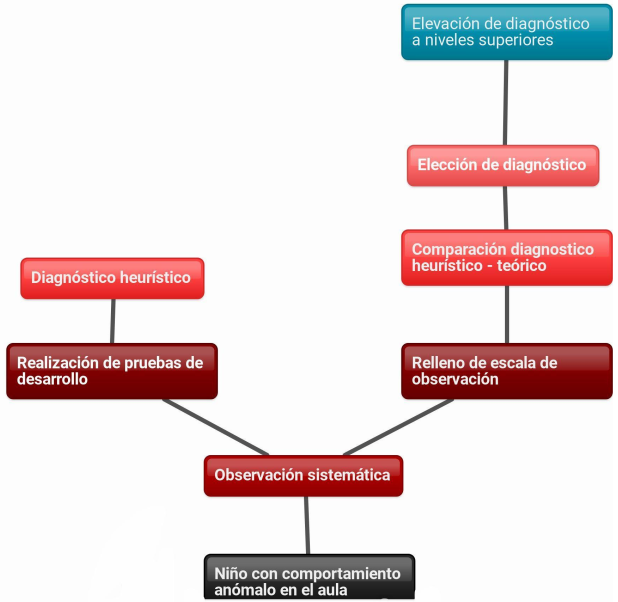
\includegraphics[width=10cm]{Pensar.png}
				\end{center}
			\end{figure}
			
\clearpage

\section{Representación del conocimiento}

Para la representación del conocimiento de este sistema experto se utiliza
un razonamiento hacia delante basado en reglas. A continuación se indican las diferentes reglas extraídas: \\

Reglas asociadas con el TDAH:
\begin{center}
\begin{tabular}{|c|}
\hline 
\textbf{Regla 1} \\ 
Si es impulsivo, \\
presta atención y \\
hace bien las tareas, entonces \\
vigilar al niño, pero no hay trastorno representativo. \\
\hline 
\end{tabular} 
\end{center}


\begin{center}
\begin{tabular}{|c|}
\hline 
 \textbf{Regla 2:} \\
Si es impulsivo, \\
presta atención, \\
hace mal las tareas y \\
sigue instrucciones, entonces \\ 
vigilar por posible TDAH. \\
\hline 
\end{tabular} 
\end{center}

\begin{center}
\begin{tabular}{|c|}
\hline 
\textbf{Regla 3:} \\
Si es impulsivo, \\ 
presta atención, \\
hace mal las tareas y \\
no sigue instrucciones, entonces \\
posible TDAH. \\
\hline 
\end{tabular} 
\end{center}

\begin{center}
\begin{tabular}{|c|}
\hline 
\textbf{Regla 4:} \\
Si es impulsivo, \\
presta atención, \\
hace mal las tareas y  \\
no sigue instrucciones, entonces \\
posible TDAH. \\
\hline 
\end{tabular} 
\end{center}

\begin{center}
	\begin{tabular}{|c|}
		\hline 
		\textbf{Regla 5:} \\
		Si es impulsivo, \\
		no presta atención y\\
		permanece sentado, entonces\\
		vigilar por posible TDAH.\\
		\hline 
	\end{tabular} 
\end{center}

\begin{center}
	\begin{tabular}{|c|}
		\hline 
		\textbf{Regla 6:} \\
		Si es impulsivo, \\
		no presta atención, \\
		permanece sentado y \\
		realiza las tareas sin problema, entonces\\
		vigilar por posible TDAH combinado. \\
		\hline 
	\end{tabular} 
\end{center}

\begin{center}
	\begin{tabular}{|c|}
		\hline 
		\textbf{Regla 7:} \\
		Si es impulsivo, \\
		no presta atención, \\
		permanece sentado y \\
		realiza las tareas con problema, entonces\\
		posible TDAH hiperactivo. \\
		\hline 
	\end{tabular} 
\end{center}

\begin{center}
	\begin{tabular}{|c|}
		\hline 
		\textbf{Regla 8:} \\
		Si no es impulsivo,\\
		presta atención y\\
		realiza las tareas sin problema, entonces\\
		no hay trastorno representativo.\\
		\hline 
		\end{tabular} 
\end{center}	
\begin{center}
	\begin{tabular}{|c|}
		\hline 
		\textbf{Regla 9:} \\
		No es impulsivo,\\
		presta atención y\\
		realiza las tareas con problema, entonces\\
		vigilar al niño\\
		\hline 
			\end{tabular} 
	\end{center}
\begin{center}
	\begin{tabular}{|c|}
		\hline 
		\textbf{Regla 10:} \\
		No es impulsivo,\\
		no presta atención,\\
		molesta en clase y\\
		realiza las tareas con problemas, entonces\\
		posible TDAH de falta de atención\\
		\hline 
		\end{tabular} 
	\end{center}
\begin{center}
	\begin{tabular}{|c|}
		\hline 
		\textbf{Regla 11:} \\
		No es impulsivo,\\
		no presta atención,\\
		molesta en clase y\\
		realiza las tareas sin problemas, entonces\\
		el niño no sufre ningún trastorno\\
		\hline 
		\end{tabular} 
	\end{center}
\begin{center}
	\begin{tabular}{|c|}
		\hline 
		\textbf{Regla 12:} \\
		No es impulsivo,\\
		no presta atención y\\
		no molesta en clase, entonces\\
		el niño no sufre ningún trastorno. \\
		\hline 
		\end{tabular} 
	\end{center}
Reglas asociadas con el trastorno Borderline:
\begin{center}
	\begin{tabular}{|c|}
		\hline 
		\textbf{Regla 13:} \\
		Lenguaje expresivo alterado, \\
		no resuelve problemas sencillos, \\
		tiene alterada la psicomotricidad y \\
		no tiene alteradas las emociones, entonces \\
		posible trastorno borderline. \\
		\hline 
	\end{tabular} 
\end{center}

\begin{center}
	\begin{tabular}{|c|}
		\hline 
		\textbf{Regla 14:} \\
		Lenguaje expresivo alterado y\\
 		resuelve problemas sencillos, entonces\\
		derivar a AL \\
		\hline 
		\end{tabular} 
	\end{center}

\begin{center}
	\begin{tabular}{|c|}
		\hline 
		\textbf{Regla 15:} \\
		Lenguaje expresivo alterado, \\
		no resuelve problemas sencillos, \\
		tiene alterada la psicomotricidad y \\
		tiene alteradas las emociones, entonces \\
		trastorno borderline. \\
		\hline 
\end{tabular} 
\end{center}

\begin{center}
	\begin{tabular}{|c|}
		\hline 
		\textbf{Regla 16:} \\
		Lenguaje expresivo alterado,\\
		no resuelve problemas sencillos,\\
		no tiene alterada la psicomotricidad y\\
		tiene alteradas las emociones, entonces\\
		trastorno retraso madurativo.\\
	\hline 
\end{tabular} 
\end{center}	
\begin{center}
	\begin{tabular}{|c|}
		\hline 
		\textbf{Regla 17:} \\
		Lenguaje expresivo alterado,\\
		no resuelve problemas sencillos,\\
		no tiene alterada la psicomotricidad, y\\
		no tiene alteradas las emociones, entonces\\
		vigilar al niño.\\
	\hline 
\end{tabular} 
\end{center}	
\begin{center}
	\begin{tabular}{|c|}
		\hline 
		\textbf{Regla 18:} \\
		Lenguaje expresivo y compresivo alterado,\\
		no resuelve problemas sencillos,\\
		tiene alterada la psicomotricidad, y\\
		tiene alteradas las emociones, entonces\\
		trastorno borderline.\\
	\hline 
\end{tabular} 
\end{center}	
\begin{center}
	\begin{tabular}{|c|}
		\hline 
		\textbf{Regla 19:} \\
		Lenguaje expresivo y compresivo alterado,\\
		no resuelve problemas sencillos,\\
		tiene alterada la psicomotricidad, y\\
		no tiene alteradas las emociones, entonces\\
		trastorno borderline.\\
	\hline 
\end{tabular} 
\end{center}	
		
\begin{center}
	\begin{tabular}{|c|}
		\hline 
		\textbf{Regla 20:} \\
		Lenguaje expresivo y compresivo alterado,\\
		no resuelve problemas sencillos,\\
		no tiene alterada la psicomotricidad, y\\
		tiene alteradas las emociones, entonces\\
		trastorno borderline.\\
	\hline 
\end{tabular} 
\end{center}	
		
\begin{center}
	\begin{tabular}{|c|}
		\hline 
		\textbf{Regla 21:} \\
		Lenguaje expresivo y compresivo alterado,\\
		no resuelve problemas sencillos,\\
		no tiene alterada la psicomotricidad, y\\
		no tiene alteradas las emociones, entonces\\
		trastorno borderline.\\
	\hline 
\end{tabular} 
\end{center}	
		
\begin{center}
	\begin{tabular}{|c|}
		\hline 
		\textbf{Regla 22:} \\
		Lenguaje expresivo y compresivo alterado,\\
		resuelve problemas sencillos,\\
		tiene alterada la psicomotricidad, y\\
		tiene alteradas las emociones, entonces\\
		vigilar, muy posible trastorno borderline.\\
	\hline 
\end{tabular} 
\end{center}	
		
\begin{center}
	\begin{tabular}{|c|}
		\hline 
		\textbf{Regla 23:} \\
		Lenguaje expresivo y compresivo alterado,\\
		resuelve problemas sencillos,\\
		tiene alterada la psicomotricidad, y\\
		no tiene alteradas las emociones, entonces\\
		derivar a AL. \\
	\hline 
\end{tabular} 
\end{center}	
		
\begin{center}
	\begin{tabular}{|c|}
		\hline 
		\textbf{Regla 24:} \\
		Lenguaje expresivo y compresivo alterado,\\
		resuelve problemas sencillos,\\
		no tiene alterada la psicomotricidad, y\\
		tiene alteradas las emociones, entonces\\
		derivar a AL.\\
	\hline 
\end{tabular} 
\end{center}	
		
\begin{center}
	\begin{tabular}{|c|}
		\hline 
		\textbf{Regla 25:} \\
		Lenguaje expresivo y compresivo alterado, \\
		resuelve problemas sencillos,\\
		no tiene alterada la psicomotricidad, y\\
		no tiene alteradas las emociones, entonces \\
		derivar a AL. \\
	\hline 
\end{tabular} 
\end{center}	

Reglas asociadas con el TEA:
\begin{center}
	\begin{tabular}{|c|}
		\hline 
		\textbf{Regla 26:} \\
		Si hace uso del lenguaje,\\
		y flexibilidad cognitiva se encuentra alterada, entonces\\
		derivar a AL\\
	\hline 
\end{tabular} 
\end{center}	
		
\begin{center}
	\begin{tabular}{|c|}
		\hline 
		\textbf{Regla 27:} \\
		Si hace uso del lenguaje,\\
		flexibilidad cognitiva no alterada,\\
		no interacciona con el entorno,\\
		mirada no perdida, y\\
		emociones irregulares, entonces\\
		vigilar por posibles caso de TEA.\\
	\hline 
\end{tabular} 
\end{center}
	
\begin{center}
	\begin{tabular}{|c|}
		\hline 
		\textbf{Regla 28:} \\
		Si hace uso del lenguaje,\\
		la flexibilidad cognitiva no alterada,\\
		no interacciona con el entorno,\\
		mirada no perdida, y\\
		emociones no irregulares, entonces\\
		vigilar por posibles caso de TEA\\
\hline 
\end{tabular} 
\end{center}

\begin{center}
	\begin{tabular}{|c|}
		\hline 
		\textbf{Regla 29:} \\
		Si hace uso del lenguaje,\\
		la flexibilidad cognitiva no esta alterada,\\
		interacciona con el entorno,\\
		tiene la mirada perdida, y\\
		buena reacción a cambios rutinarios, entonces\\
		derivar a AL\\
\hline 
\end{tabular} 
\end{center}	
		
\begin{center}
	\begin{tabular}{|c|}
		\hline 
		\textbf{Regla 30:} \\
		Si hace uso del lenguaje,\\
		la flexibilidad cognitiva no esta alterada,\\
		interacciona con el entorno,\\
		tiene la mirada perdida, y\\
		mala reacción a cambios rutinarios, entonces\\
		posible caso de TEA\\
\hline 
\end{tabular} 
\end{center}
		
\begin{center}
	\begin{tabular}{|c|}
		\hline 
		\textbf{Regla 31:} \\
		Si hace uso del lenguaje,\\
		la flexibilidad cognitiva no esta alterada,\\
		interacciona con el entorno,\\
		no tiene la mirada perdida, y\\
		no tiene emociones irregulares, entonces\\
		no presenta trastorno pero vigilar.\\
\hline 
\end{tabular} 
\end{center}
		
\begin{center}
	\begin{tabular}{|c|}
		\hline 
		\textbf{Regla 32:} \\
Si hace uso del lenguaje,\\
la flex cognitiva no esta alterada,\\
interacciona con el entorno,\\
no tiene la mirada perdida,\\
tiene emociones irregulares,\\
derivar a AL.\\
\hline 
\end{tabular} 
\end{center}
	
\begin{center}
	\begin{tabular}{|c|}
		\hline 
		\textbf{Regla 33:} \\
Si hace uso del lenguaje,
la flexibilidad cognitiva no esta alterada,\\
no interacciona con el entorno,\\
tiene la mirada perdida\\
tiene emociones irregulares, y\\
presenta empatía, entonces\\
vigilar por posible caso de TEA\\
\hline 
\end{tabular} 
\end{center}

\begin{center}
	\begin{tabular}{|c|}
		\hline 
		\textbf{Regla 34:} \\
		Si hace uso del lenguaje,\\
		la flexibilidad cognitiva no esta alterada,\\
		no interacciona con el entorno,\\
		tiene la mirada perdida\\
		tiene emociones irregulares, y\\
		no presenta empatía, entonces\\
		derivar a AL\\
\hline 
\end{tabular} 
\end{center}
		
\begin{center}
	\begin{tabular}{|c|}
		\hline 
		\textbf{Regla 35:} \\
		Si hace uso del lenguaje,\\
		la flexibilidad cognitiva no esta alterada,\\
		no interacciona con el entorno,\\
		tiene la mirada perdida, y\\
		no tiene emociones irregulares, entonces\\
		el niño no presenta ningún trastorno.\\
\hline 
\end{tabular} 
\end{center}
		
\begin{center}
	\begin{tabular}{|c|}
		\hline 
		\textbf{Regla 36:} \\
		Si no hace uso del lenguaje,\\
		la flexibilidad cognitiva no esta alterada,\\
		no interacciona con el entorno,\\
		tiene la mirada perdida,\\
		y sus emociones están alteradas, entonces\\
		el niño presenta TEA y derivar a PT\\
\hline 
\end{tabular} 
\end{center}		
		
\begin{center}
	\begin{tabular}{|c|}
		\hline 
		\textbf{Regla 37:} \\
		Si no hace uso del lenguaje,\\
		la flexibilidad cognitiva no esta alterada,\\
		no interacciona con el entorno,\\
		tiene la mirada perdida,\\
		y sus emociones no están alteradas, entonces\\
		vigilar como posible caso de TEA.\\
\hline 
\end{tabular} 
\end{center}		
		
\begin{center}
	\begin{tabular}{|c|}
		\hline 
		\textbf{Regla 38:} \\
		Si no hace uso del lenguaje,\\
		la flexibilidad cognitiva no esta alterada,\\
		no interacciona con el entorno,\\
		no tiene la mirada perdida,\\
		y sus emociones están alteradas, entonces\\
		vigilar como posible caso de TEA.\\
\hline 
\end{tabular} 
\end{center}		
		
\begin{center}
	\begin{tabular}{|c|}
		\hline 
		\textbf{Regla 39:} \\
		Si no hace uso del lenguaje,\\
		la flexibilidad cognitiva no esta alterada,\\
		no interacciona con el entorno,\\
		no tiene la mirada perdida,\\
		y sus emociones no están alteradas, entonces\\
		vigilar como posible caso de TEA.\\
\hline 
\end{tabular} 
\end{center}		
		
\begin{center}
	\begin{tabular}{|c|}
		\hline 
		\textbf{Regla 40:} \\
		Si no hace uso del lenguaje,\\
		la flexibilidad cognitiva no esta alterada, y\\
		interacciona con el entorno, entonces\\
		el niño no sufre TEA, derivar a AL.\\
\hline 
\end{tabular} 
\end{center}		
		
\begin{center}
	\begin{tabular}{|c|}
		\hline 
		\textbf{Regla 41:} \\
		Si no hace uso del lenguaje, y\\
		la flexibilidad cognitiva esta alterada , entonces \\
		posible caso de TEA. \\
\hline 
\end{tabular} 
\end{center}
\newpage
\section{Relaciones borrosas}
\begin{figure}[h!]
	\begin{subfigure}
		\includegraphics[width=8cm]{"Documento 6(1)_page-0001"}
	\end{subfigure}
	\hfill
	\begin{subfigure}
		\includegraphics[width=8.2cm]{"Foto_page-0001"}
	\end{subfigure}
\end{figure}
\newpage
\section{Control borroso}
Conjuntos borrosos, se ha utilizado la regla nombrada anteriormente para la creación de este ejemplo.

\begin{figure}[h!]
	\begin{subfigure}
		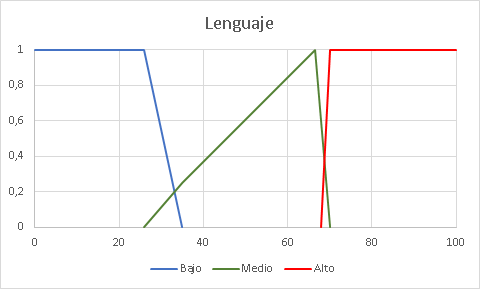
\includegraphics[width=8cm]{Lenguaje.png}
	\end{subfigure}
	\hfill
	\begin{subfigure}
		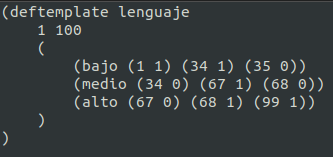
\includegraphics[width=7cm]{lengu.png}
	\end{subfigure}
\end{figure}

\begin{figure}[h!]
	\begin{subfigure}
		\includegraphics[width=7cm]{Flex.cogni.png}
	\end{subfigure}
	\hfill
	\begin{subfigure}
		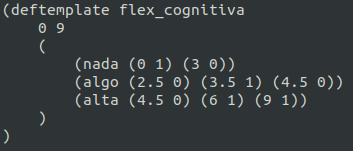
\includegraphics[width=7cm]{flex.png}
	\end{subfigure}
\end{figure}

\begin{figure}[h!]
	\begin{subfigure}
		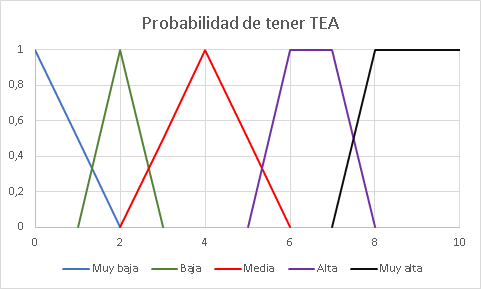
\includegraphics[width=7cm]{probabilidad.png}
	\end{subfigure}
	\hfill
	\begin{subfigure}
		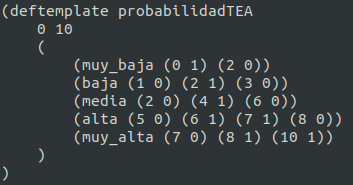
\includegraphics[width=7cm]{prob.png}
	\end{subfigure}
\end{figure}
 \newpage
\subsection{Reglas construidas}
\begin{figure}[htb]
	\begin{center}
		\includegraphics[width=13.5cm]{Reglas.png}
	\end{center}
\end{figure}

(defrule regla\_1
(lenguaje bajo)
(flex\_cognitiva algo)
= \textgreater
(assert (probabilidadTEA baja))
)

(defrule regla\_2
(lenguaje bajo)
(flex\_cognitiva nada)
=\textgreater
(assert (probabilidadTEA muy\_baja))
)

(defrule regla\_3
(lenguaje bajo)
(flex\_cognitiva alta)
=\textgreater
(assert (probabilidadTEA media))
)

(defrule regla\_4
(lenguaje medio)
(flex\_cognitiva nada)
=\textgreater
(assert (probabilidadTEA baja))
)

(defrule regla\_5
(lenguaje medio)
(flex\_cognitiva algo)
=\textgreater
(assert (probabilidadTEA media))
)

(defrule regla\_6
(lenguaje medio)
(flex\_cognitiva alta)
=\textgreater
(assert (probabilidadTEA alta))
)

(defrule regla\_7
(lenguaje alto)
(flex\_cognitiva nada)
=\textgreater
(assert (probabilidadTEA media))
)

(defrule regla\_8
(lenguaje alto)
(flex\_cognitiva algo)
=\textgreater
(assert (probabilidadTEA alta))
)

(defrule regla\_9
(lenguaje alto)
(flex\_cognitiva alta)
=\textgreater
(assert (probabilidadTEA muy\_alta))
)

\newpage
\subsection{Ejemplo Mamdani}
Hecho utilizado: \\
(deffacts hecho
\\
(lenguaje (26.5 0) (26.5 1) (26.5 0))
\\
(flex\_cognitiva (4 0) (4 1) (4 0))
\\
) \\

Obtención realizada a \textbf{mano}: 
\begin{figure}[h!]
	\begin{center}
		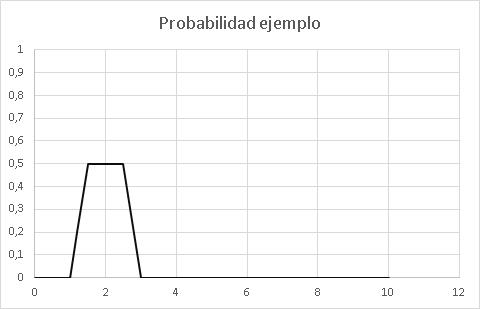
\includegraphics[width=8cm]{ProbabilidadEjemplo.png}
	\end{center}
\end{figure} 
\newpage
Obtención de resultado con \textbf{fuzzyclips}: 
\begin{figure}[h!]
	\centering
	\includegraphics[width=0.7\linewidth]{mamdani}
\end{figure} \\
\textbf{Deborrosificación}
\begin{figure}
	\centering
	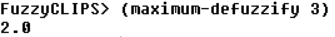
\includegraphics[width=0.4\linewidth]{defuzzify}
\end{figure}
 \newpage
\section{Conclusión}
\textbf{Problemas encontrados} \\
Uno de los mayores problemas que se encontraron durante la realización de este trabajo fue la gran cantidad de información, al ser un prototipo tuve que definir muy bien los limites que finalmente alcanzaría. \\

Otro de los problemas que encontré fue el gran número de comportamientos por trastorno, aun así creo que el prototipo final es bastante escalable pudiendo llegar a un sistema experto mayor. La definición de estos trastornos con sus comportamientos no habría sido posible sin la dedicación de los expertos que me ayudaron en todo momento y me aportaron gran cantidad de información. \\

\textbf{Utilidades encontradas} \\
Una vez finalizado llego el turno de enseñarlo a los expertos para dar unos últimos retoques, al no ser profesionales de la informática les resulto un tanto peculiar ver un programa como nosotros estamos acostumbrados pero quedaron bastante satisfechos con el resultado y preguntaron por hacerlo aun más grande. \\

\textbf{Sobre lo aprendido en la asignatura} \\
Creo que es un proyecto bastante grande y muy entretenido de realizar, desde el punto de vista estudiantil he aprendido mucho, creo que lo más interesante fue todo lo que concierne a la lógica borrosa. Por otro lado, me ha ayudado a acercarme a otras ciencias y poder unirlas con la informática, esto ultimo me resulta muy importante ya que considero que se debería trabajar más y no individualizar la ciencia.


\end{document}